% \begin{spverbatim}
%1st paragraph
%1
\revised{3D data is acquired using the system presented by Akiyama et al. and Li et al. \cite{9789786,9507455}.}
\deleted{In the proposed system, 3D data is acquired using the system presented by Akiyama et al. and Li et al. \cite{9789786,9507455}.}
  %1-1
  \revised{Multiple LiDAR calibrations merge streams by rotating and translating 3D data according to predetermined angles and distances.}
  \begin{deletedblock}
  Multiple LiDAR calibrations are performed for merging and the angles and distances are determined. 
    The axis of the 3D data is rotated based on the angles, and the 3D data is translated based on the distances.
  \end{deletedblock}

%2nd paragraph
%2
The point cloud of each frame of the aggregated 3D data is trimmed.
  %2-1
  \revised{Vertices of each person's region are determined manually under a fixed-seating office layout.}
  \begin{deletedblock}
  Here, the coordinates of the vertices of a region where a person is located are determined manually, and the region is cut out. 
    The manual determination assumes a fixed-seating office environment, where the location of each person's workspace is pre-determined and known in advance.
  \end{deletedblock}

%3rd paragraph
%3
\revised{Four feature types were selected to capture complementary geometric properties of hand-region point clouds.}
  %3-1
  \revised{Normals encode local surface orientation of hands and forearms.}
  %3-2
  \revised{Dimensionality features distinguish linear, planar, and volumetric local structures.}
  %3-3
  \revised{Proportion of variance summarizes eigenvalue distribution within each neighborhood.}
  %3-4
  \revised{FPFH encodes pairwise angular relationships among neighboring points.}
%4
Four types of features are extracted from the trimmed point clouds: normals, dimensionality features, proportion of variance, and FPFH. 
  %4-1
  \revised{For normals, dimensionality features, and proportion of variance, the k-nearest neighbor algorithm (KNN) uses search radius 100 and maximum 30 neighbors to build covariance matrices at each point.}
  \deleted{The k-nearest neighbor algorithm (KNN) is implemented using the determined parameters.}
  %4-2
  \textit{Normals.} 
    %4-2-1
    \revised{Eigenvectors of the smallest eigenvalue in each covariance matrix serve as normals (Fig.~\ref{features}\subref{normal}).}
    \begin{deletedblock}
      The search radius was 100. 
      The maximum number of neighbors was 30. 
    Covariance matrices are generated from each point in the point cloud based on KNN. 
    Eigenvectors corresponding to the smallest eigenvalue in the covariance matrices are used as the normals. 
    Fig.~\ref{features}\subref{normal} shows the data with the normals. 
    \end{deletedblock}
  %4-3
  \textit{Dimensionality features} \cite{isprs-archives-XXXVIII-5-W12-97-2011,YANG201319}.
    %4-3-1
    \revised{Eigenvalues ${\lambda}_i$, $i=[1, 3]$ yield $a_{1D}=\frac{\sqrt{{\lambda}_1}-\sqrt{{\lambda}_2}}{\sqrt{{\lambda}_1}}$, $a_{2D}=\frac{\sqrt{{\lambda}_2}-\sqrt{{\lambda}_3}}{\sqrt{{\lambda}_1}}$, and $a_{3D}=\frac{\sqrt{{\lambda}_3}}{\sqrt{{\lambda}_1}}$ \cite{isprs-archives-XXXVIII-5-W12-97-2011,YANG201319} (Fig.~\ref{features}\subref{dimensionality}).}
    \begin{deletedblock}
    KNN is performed using the determined parameters. 
    Covariance matrices are generated from each point in the point cloud based on KNN. 
    Eigenvalues are defined as ${\lambda}_i$, $i=[1, 3]$ and the dimensionality features are calculated as $a_{1D}=\frac{\sqrt{{\lambda}_1}-\sqrt{{\lambda}_2}}{\sqrt{{\lambda}_1}}$, $a_{2D}=\frac{\sqrt{{\lambda}_2}-\sqrt{{\lambda}_3}}{\sqrt{{\lambda}_1}}$, and $a_{3D}=\frac{\sqrt{{\lambda}_3}}{\sqrt{{\lambda}_1}}$\cite{isprs-archives-XXXVIII-5-W12-97-2011,YANG201319}. 
    Fig.~\ref{features}\subref{dimensionality} shows the data with the dimensionality features. 
    \end{deletedblock}
  %4-4
  \textit{Proportion of variance} \cite{BRODU2012121}. 
    %4-4-1
    \revised{Proportion of variance is $\boldsymbol{v_i}=\frac{{\lambda}_i}{{\lambda}_1+{\lambda}_2+{\lambda}_3}(i=[1, 3])$ (Fig.~\ref{features}\subref{proportion}).}
    \begin{deletedblock}
    KNN is performed using the determined parameters. 
    Covariance matrices are generated from each point in the point cloud based on the KNN. 
    Eigenvalues are defined as ${\lambda}_i$, $i=[1, 3]$ and the proportion of variance is calculated as $\boldsymbol{v_i}=\frac{{\lambda}_i}{{\lambda}_1+{\lambda}_2+{\lambda}_3}(i=[1, 3])$. 
    Fig.~\ref{features}\subref{proportion} shows the data with the proportion of variance. 
    \end{deletedblock}
  %4-5
  \textit{FPFH} \cite{5152473}. 
    %4-5-1
    \revised{Two adjacent points per center point define a Darboux frame; FPFH is computed from frame-based angular relations and concatenated; principal component analysis (PCA) with randomized singular value decomposition reduces the 33-dimensional FPFH to three dimensions (Fig.~\ref{features}\subref{fpfh}).}
    \begin{deletedblock}
    Two points in a set of points adjacent to each point in the point cloud are chosen on the basis of the parameters \cite{4795593,4650967}. 
    The Darboux frame $u$, $v$, and $w$ are defined by using the two points and normals. 
    Three variables are defined. 
      The first variable is a dot product vector between the one of the normal and the frame $v$. 
      The second variable is a unit vector of a dot product vector between the one of a distance vector of two points and the frame $v$. 
      The third variable is an arctangent function consisting of a dot product vector between the one of the normal and the frame $u$, and a dot product vector between the one of the normal and the frame $w$. 
      The FPFH is generated from combinations of a center point and the surrounding points in the point cloud and then several FPFHs are concatenated. 
    PCA is used to reduce the dimensions of the FPFH. 
      PCA is used to reduce the 33-dimensional FPFH to three dimensions.
      The randomized SVD solver is used. 
    Fig.~\ref{features}\subref{fpfh} shows the data with the FPFH. 
    \end{deletedblock}

%4th paragraph
%5
Next, clustering is performed for the point clouds using the point features. 
  %5-1
  \revised{DBSCAN ($\varepsilon=100$, minimum 10 points on 3D coordinates) and k-means ($k=3$) each remove outliers and extraneous clusters \cite{ester1996density,hartigan1979algorithm}.}
  %5-2
  \revised{DBSCAN removes isolated noise points from background objects and sensor reflections.}
  %5-3
  \revised{k-means partitions the point cloud into fixed spatial groups; extraneous partitions are discarded.}
  %5-4
  \revised{Aggressive cluster removal can delete sparse finger points and degrade classification of fine hand postures.}
  \begin{deletedblock}
  DBSCAN is used to determine the parameters for DBSCAN so as to remove noise in the point cloud and then align circles to each point in the point cloud on the basis of the parameters \cite{ester1996density}.
      The neighborhood radius $\varepsilon$ is 100. 
      The minimum number of points is 10. 
      DBSCAN is applied to the three-dimensional coordinates of each point. 
    Points that have more than a certain number of points in the circle centered at the point are defined as ``core'' and points within the radii of the circles that the cores have are defined as ``reachable points''. 
    Points that are not near to any cores are considered outliers. 
    The outliers and some of the clusters are removed. 
  k-means is used to determine the number of clusters for k-means so as to remove noise in the point cloud \cite{hartigan1979algorithm}. 
    The number of clusters $k$ was 3.
    Each point in the point cloud is randomly assigned to a cluster, and as long as the cluster changes, the following process is repeated. 
      Specifically, the centroids of each cluster are determined and the cluster to which each point belongs is changed in accordance with the nearest center of the centroids. 
    The outliers and some of the clusters are removed. 
  \end{deletedblock}

%5th paragraph
%6
Downsampling is performed for the clustered point clouds. 

%6th paragraph
%7
\revised{Downsampled training point clouds are normalized so that the distance from the center of gravity to the farthest point equals 1.0.}
\begin{deletedblock}
Normalization is performed for the downsampled point clouds for the training data. 
  Here, 1.0 is set as the distance from the center of gravity to the farthest point. 
  The downsampled point clouds are normalized on the basis of this distance. 
\end{deletedblock}

%7th paragraph
%8
\revised{PointNet++ classifies normalized point clouds by repeatedly selecting points, grouping neighborhoods, and processing each group with PointNet and a fully connected layer \cite{DBLP:journals/corr/QiYSG17}.}
  %8-1
  \revised{Two-level grouping in PointNet++ captures hand-scale local structures that distinguish mouse operation, pad operation, typing, and sitting still.}
\deleted{Classification is performed for the normalized point clouds utilizing PointNet++ to determine the parameters for PointNet++ so as to determine size of the data to process \cite{DBLP:journals/corr/QiYSG17}.}
  \deleted{The following process is repeated twice: a few points in each point cloud are first chosen, a group formed from each selected point and the surrounding points is created, and then each group is processed using PointNet and a fully connected layer.}

% \end{spverbatim}
%6/27 tb ⇒ t
\begin{deletedblock}
\begin{figure}[t]
  \centering
  {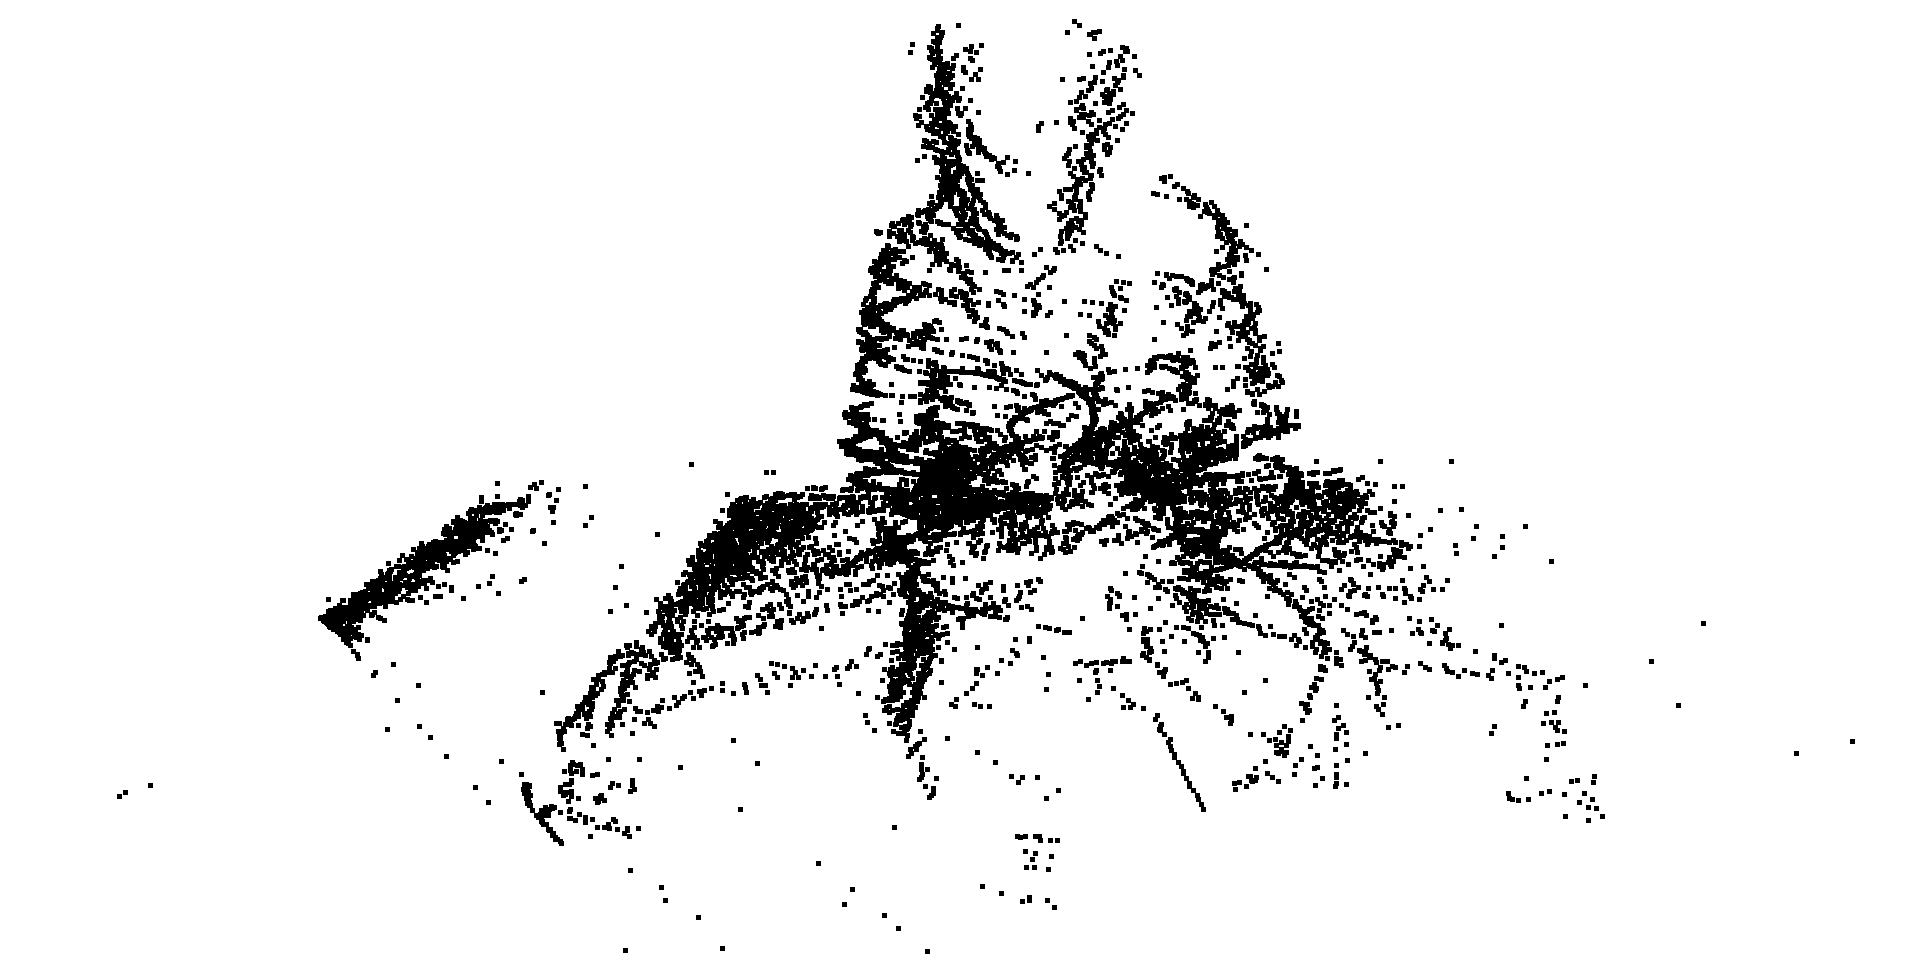
\includegraphics[width=\linewidth]{img/cutdata.png}}
  \caption{Trimmed data.}
  \label{trimdata}
\end{figure}
\end{deletedblock}

%6/27 tb ⇒ t
\begin{figure}[t]
  \centering
  \subfloat[Normals]{
    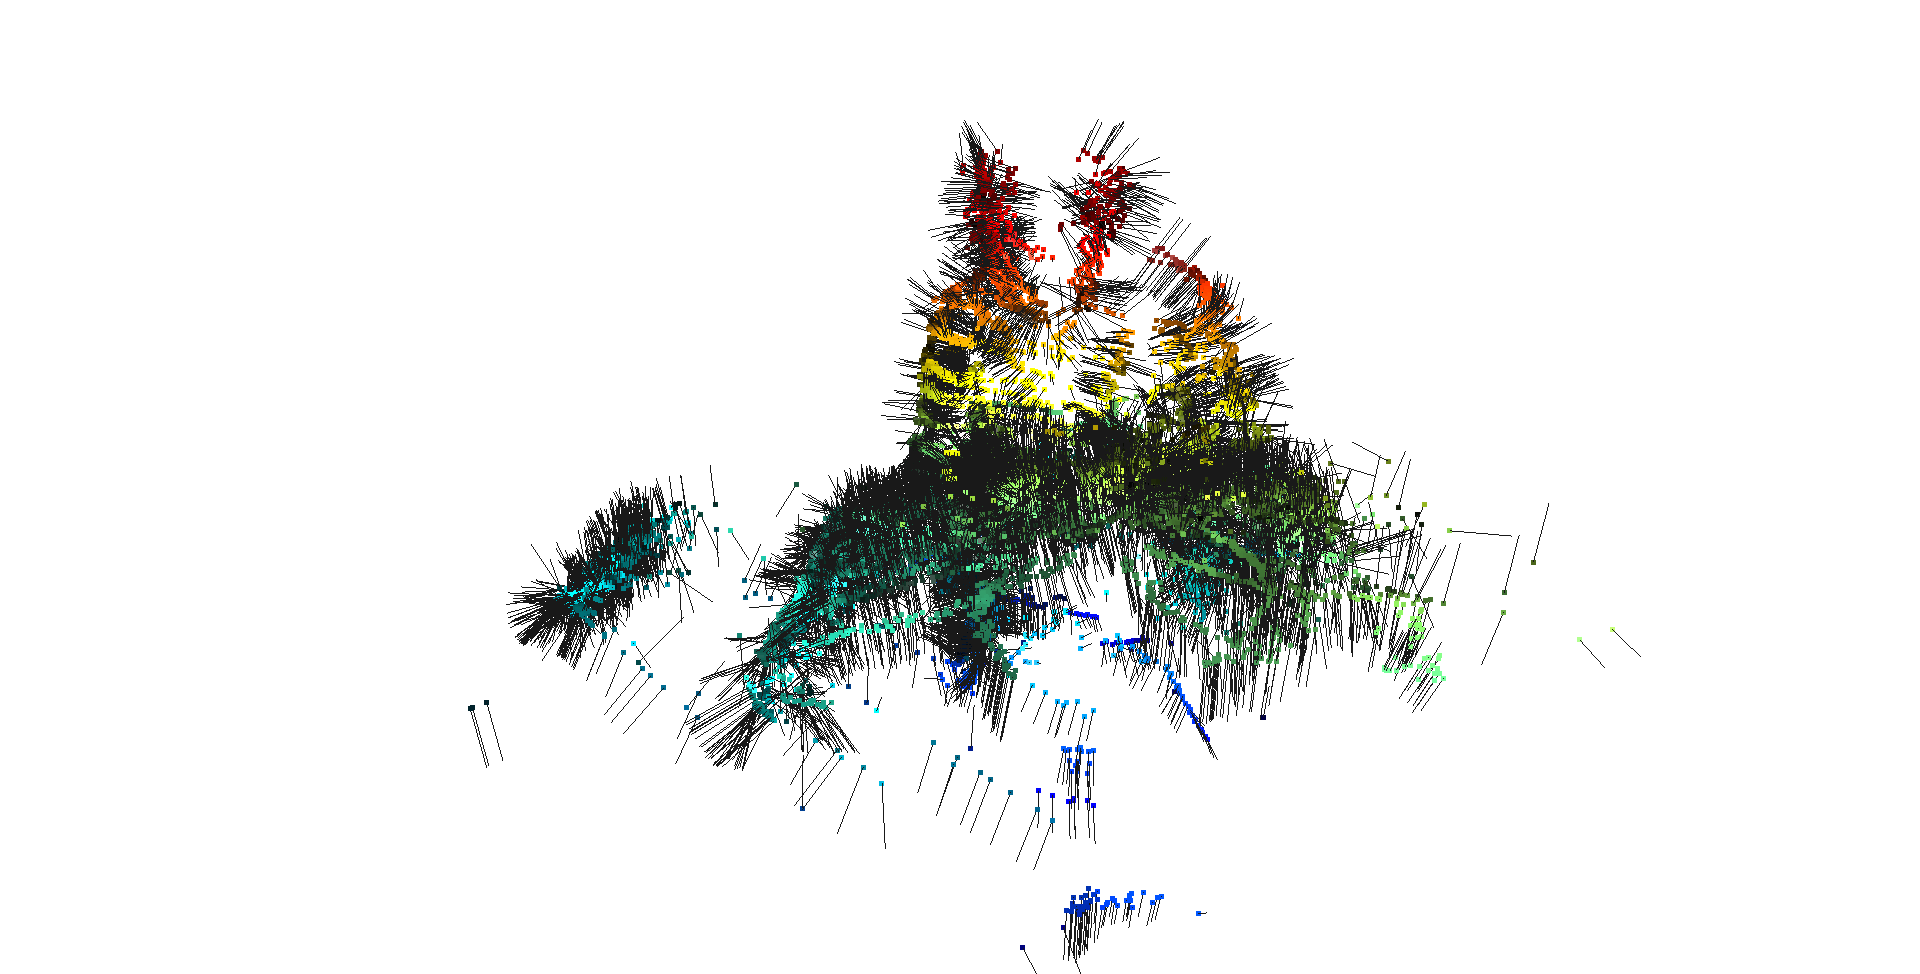
\includegraphics[width=.45\linewidth]{img/normal.png}
    \label{normal}
  }
  \subfloat[Dimensionality features]{
    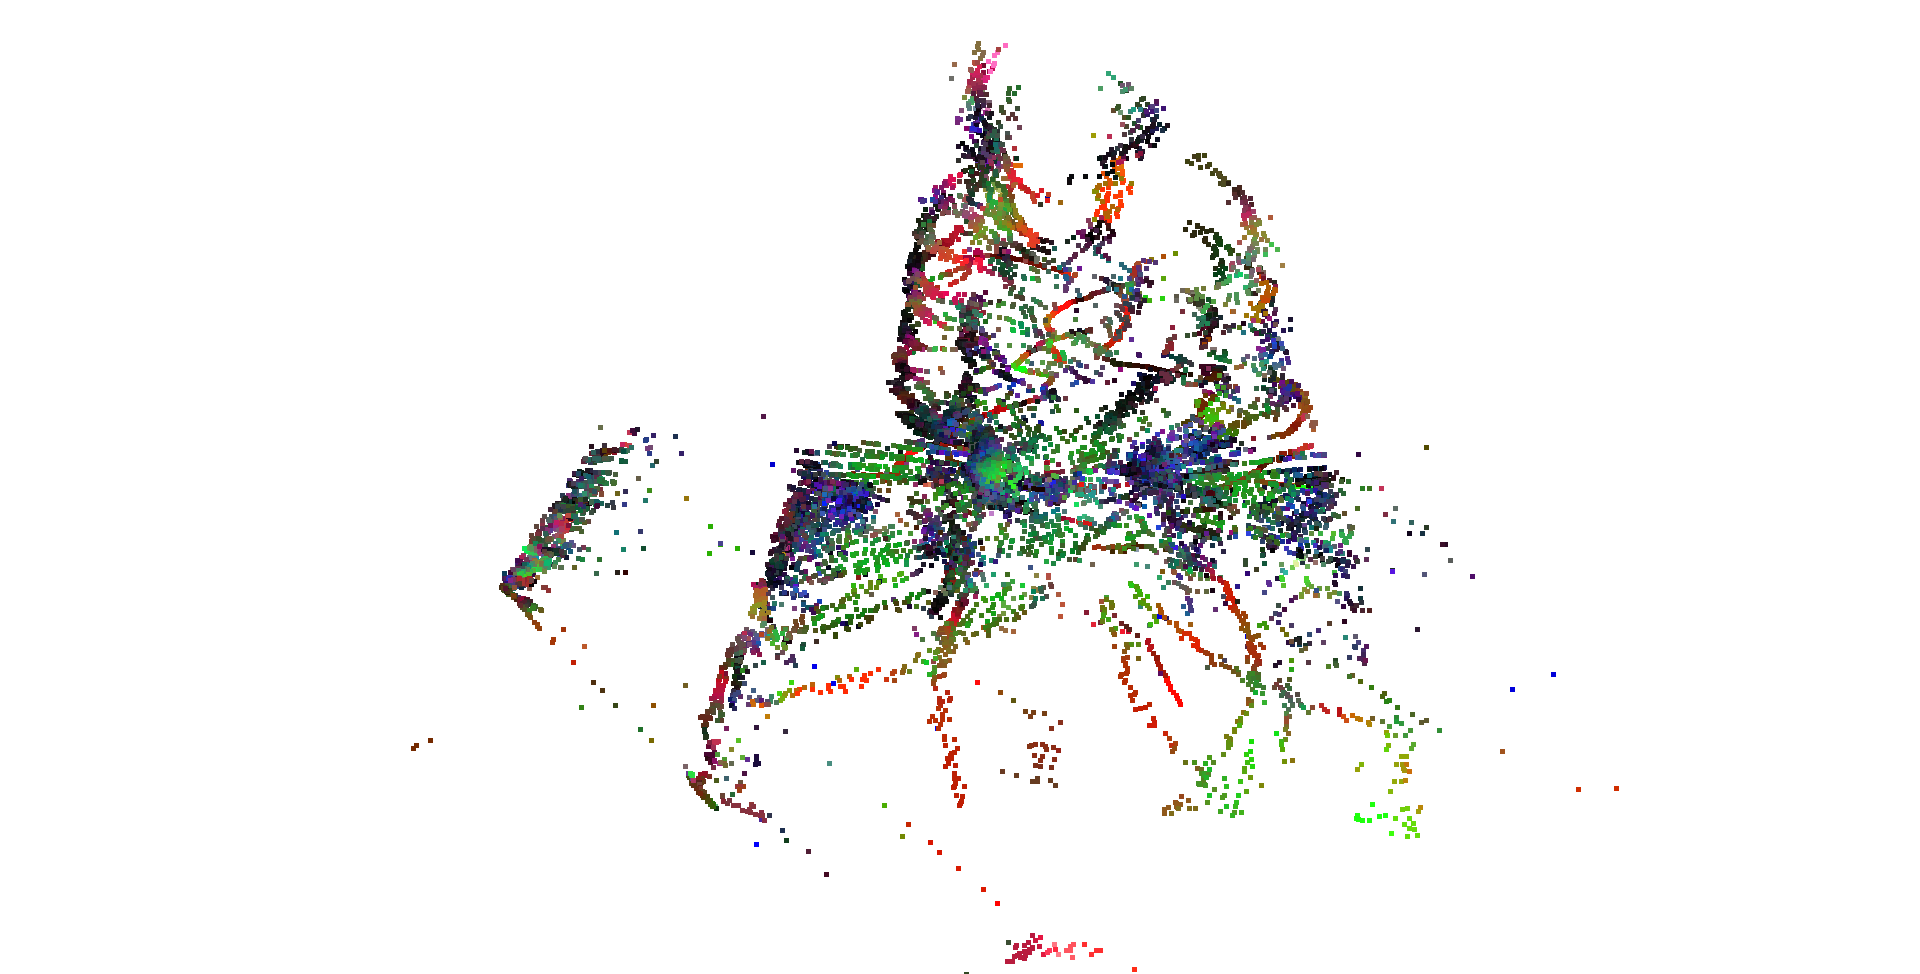
\includegraphics[width=.45\linewidth]{img/dim.png}
    \label{dimensionality}
  }
  \\
  \subfloat[Proportion of variances]{
    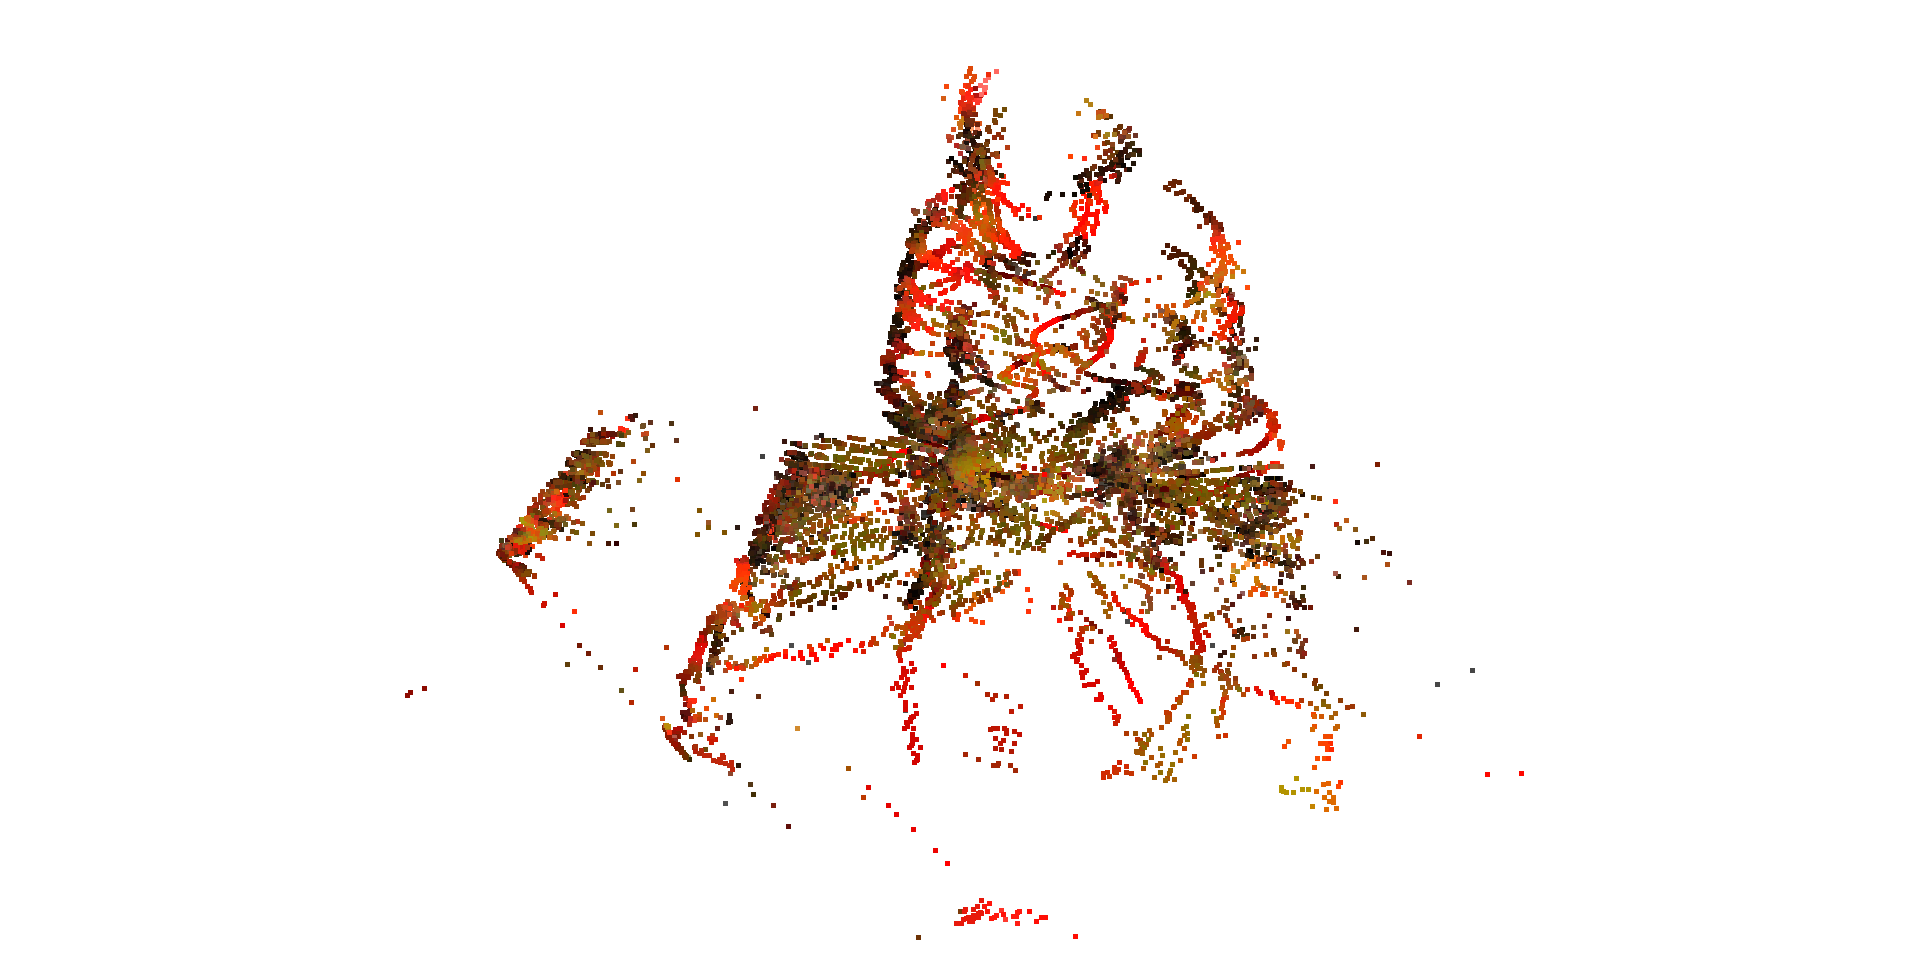
\includegraphics[width=.45\linewidth]{img/proportion.png}
    \label{proportion}
  }
  \subfloat[FPFH]{
    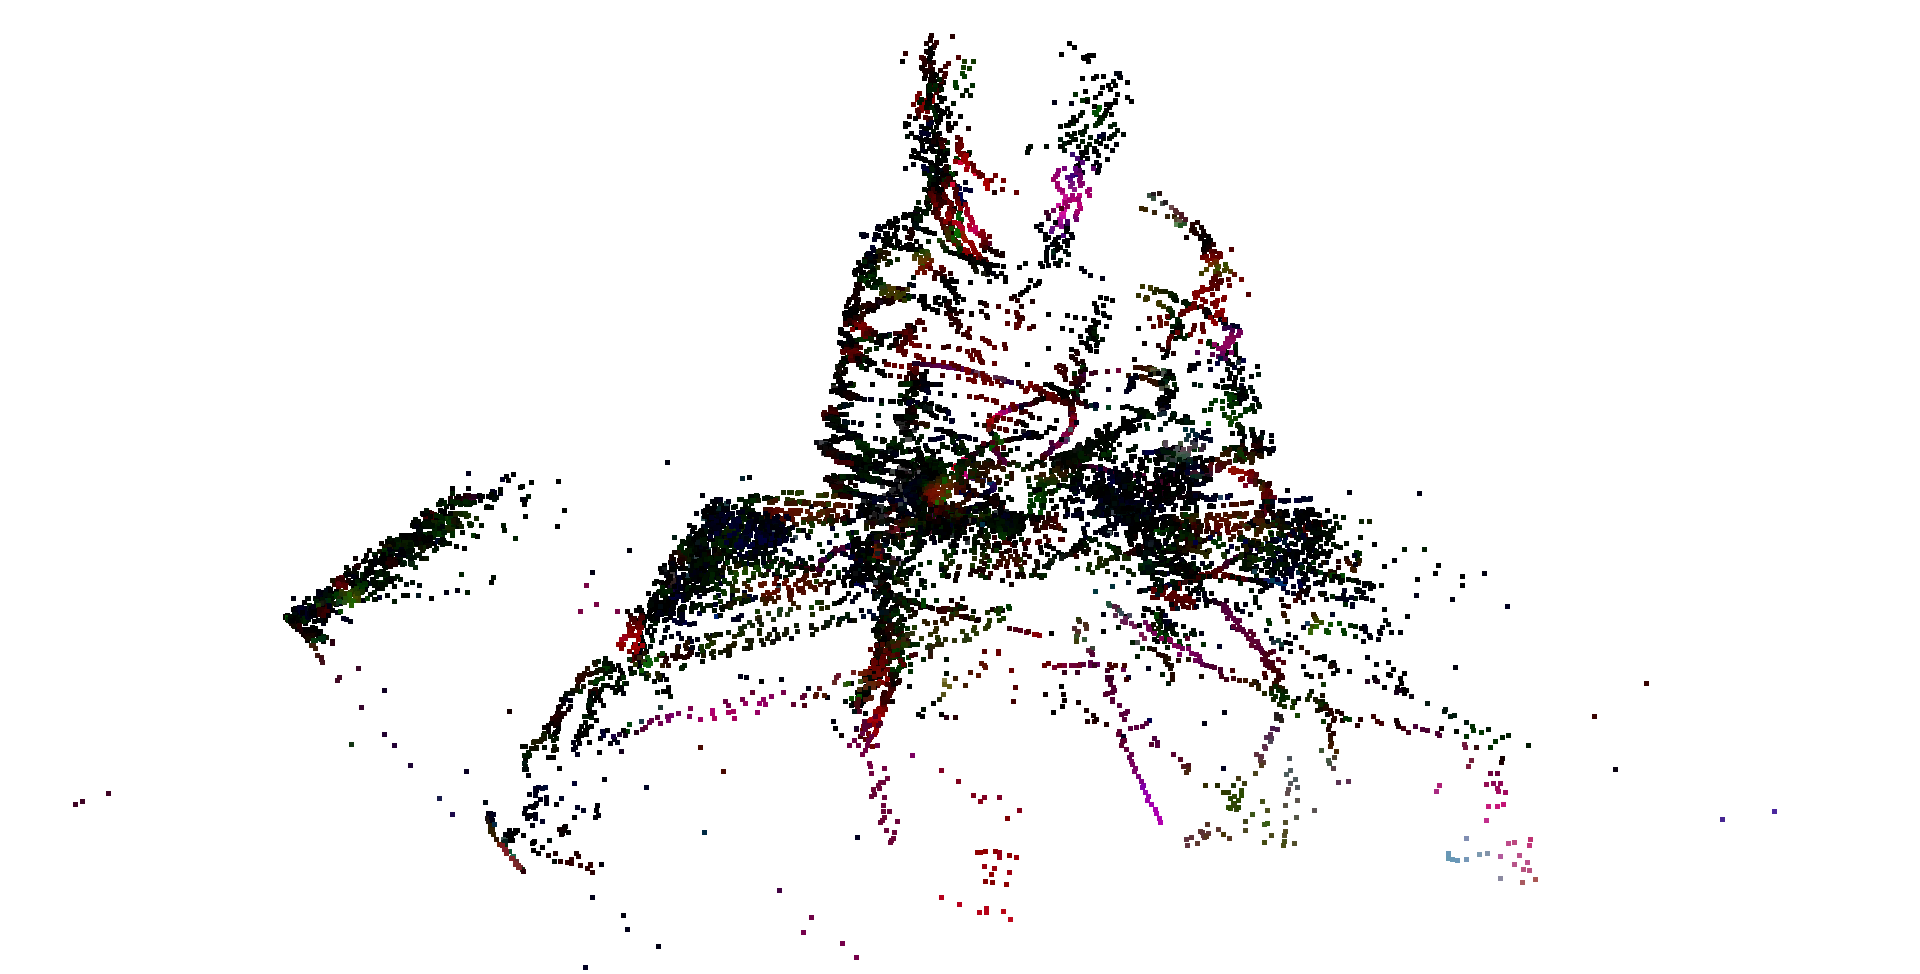
\includegraphics[width=.45\linewidth]{img/fpfh.png}
    \label{fpfh}
  }
  \caption{Point clouds with each of four types of feature.}
  \label{features}
\end{figure}
